%%%\scalebox{1.2}{ 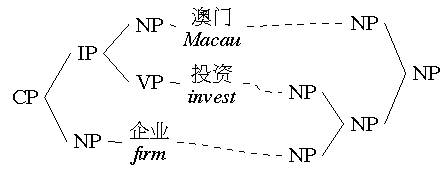
\includegraphics{figures/chinese-tree1} }

\begin{tikzpicture}
\tikzset{every tree node/.style={align=center}}
\Tree
[.\extranode{NP}
  [.NP 澳门\\Macau ]
  [.\extranode{NP}
    [.\extranode{NP} 投资\\invest ]
    [.NP 企业\\firm ] ] ]
\end{tikzpicture}

\vspace{3mm}
(a) Parser output

\vspace{6mm}

\begin{tikzpicture}
\tikzset{every tree node/.style={align=center}}
\Tree
[.\missingnode{CP}
  [.\missingnode{IP}
    [.NP 澳门\\Macau ]
    [.\missingnode{VP} 投资\\invest ] ]
  [.NP 企业\\firm ] ]
\end{tikzpicture}

\vspace{3mm}
(b) Gold parse
\derivspace
\caption[Error analysis example: Word sense confusion (Chinese).]{ \label{fig:sense} 
  \textbf{Sense Confusion} By treating \glos{投资}{invest} as a noun, the parser forms an NP about a type of firm, rather than a clause about action by \Trans{Macau}.
}
